\section{Funkcje wielu zmiennych}

Na początek kilka definicji dotyczących zbiorów w $ \mathbb{R}^n $.

\begin{tw}{Definicja}
    \underline{Otoczenie} punktu $ P = (x_1, x_2, ..., x_n) \in \mathbb{R}^n $ to $n$ -- wymiarowa kula otwarta o środku
    w $P$ i promieniu $r > 0$, tzn. zbiór
    \[ K(P, r) = \{ Q = (y_1, y_2, ..., y_n) \in \mathbb{R}^n : |PQ|^2 = (x_1 - y_1)^2 + (x_2 - y_2)^2 + ... + (x_n - y_n)^2 < r^2 \} \]
    
    Dla $n=2$ jest to koło o środku w $P$ bez brzegowego okręgu.
    
    Dla $n=3$ jest to kula o środku w $P$ bez brzegowej sfery.
\end{tw}
\begin{tw}{Definicja}
    
\underline{Sąsiedztwo} punktu $x_0 \in \mathbb{R}^n$ to zbiór postaci $ S = S(P, r) = K(P,r) \backslash P $
    Zbiór $ A \subset \mathbb{R}^n $ jest zbiorem \underline{otwartym}, gdy każdy punkt z $A$ posiada pewne otoczenie zawarte w $A$, tzn.
    \[ \forall P \!\in\! A \ \exists K(P, r) \quad P\in K(P,r) \subset A \]
    Zbiór $ A \subset \mathbb{R}^n $ jest zbiorem \underline{domkniętym}, gdy jego dopełnienie $ A = \mathbb{R}^n \backslash A $ jest zbiorem otwartym.
\end{tw}

\begin{tw}{Definicja}

Funkcja wielu zmiennych ma postać
$$ f: D \to \mathbb{R} $$
gdzie $ D \subset \mathbb{R}^n $ jest dziedziną $f$.

Zatem dla $ (x_1, x_2, ..., x_n) \in D $ \quad $ f(x_1, x_2, ..., x_n) \in \mathbb{R} $
\end{tw}

Gdy mamy funkcje dwóch zmiennych to zwykle piszemy $ z = f(x, y) $ a dla trzech zmiennych $ t = f(x, y, z) $.

Będziemy analizować głównie funkcje dwóch zmiennych $ z = f(x, y) $.

Dla takich funkcji można narysować wykres -- gdy $D$ jest otwarty to wykresem jest powierzchnia w $3$ wymiarach dana wzorem
$ (x, y, f(x,y)) $, gdzie $ (x,y) \in D_f $.

\begin{center}
    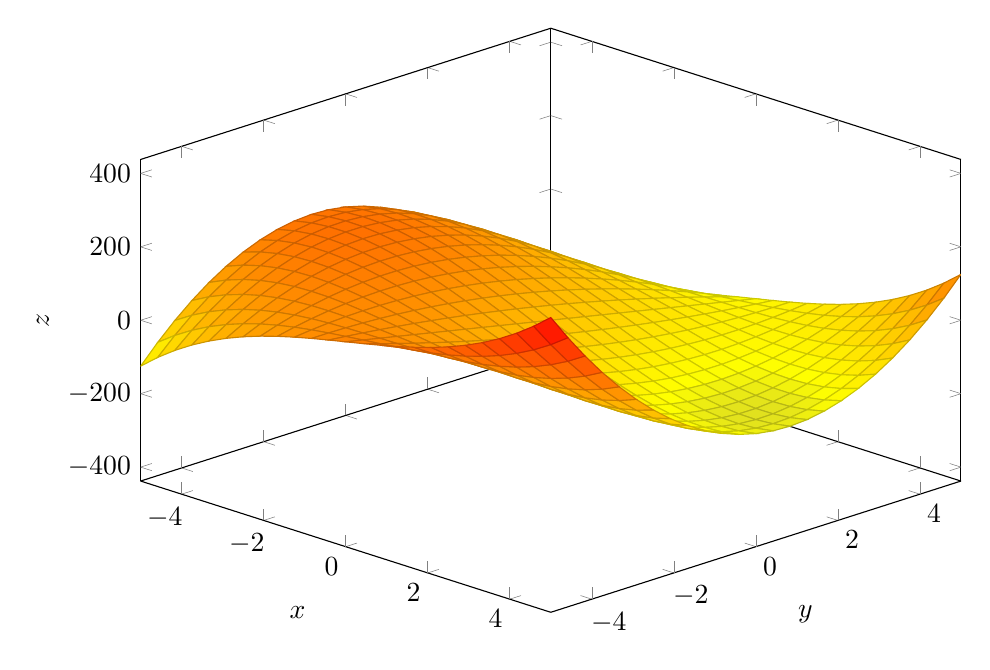
\begin{tikzpicture}
        \begin{axis}[
            width=12cm, height=9cm,
            view={45}{30},
            xlabel={$x$}, ylabel={$y$}, zlabel={$z$},
            xmin=-5, xmax=5,
            ymin=-5, ymax=5,
            ]
            \addplot3[surf]{x^3 + 3*x*y^2 - 51*x - 24*y};            
        \end{axis}
    \end{tikzpicture}

Wykres funkcji $ f(x,y) = x^3 + 3xy^2 - 51x - 24y, \quad -5 \leq x \leq 5, \ -5 \leq y \leq 5 $
\end{center}

\textbf{Wykresy niektórych popularnych funkcji}

\begin{itemize}
    \item $ z = Ax + By + C $ -- płaszczyzna o wektorze normalnym $ \vec{n} = [A, B, -1] $ i przechodząca przez punkt $ (0,0,C) $.
    \item $ z = z_0 + \sqrt{r^2 - (x-x_0)^2 - (y-y_0)^2} $ -- górna półsfera o środku w $(x_0, y_0, z_0)$ i promieniu $r > 0$. Np.
    $ z = 3 + \sqrt{7 - x^2 - (y-1)^2} : \ S(0,1,3), \ r=\sqrt{7} $

    $ z = z_0 - \sqrt{r^2 - (x-x_0)^2 - (y-y_0)^2} $ -- analogiczna półsfera ale dolna.

    Obie pochodzą z równania całej sfery: $ (x - x_0)^2 + (y - y_0)^2 + (z - z_0)^2 = r^2 $.
    \item $ z = z_0 + a\sqrt{(x-x_0)^2 + (y-y_0)^2}, \ a \neq 0 $ -- powierzchnia stożkowa o wierzchołku w $ P = (x_0,y_0,z_0) $
    i osi symetrii równoległej do osi $Z$.

    $a > 0$ -- wierzchołek w dół, $a < 0$ -- wierzchołek w górę.

    $|a| = \tan \alpha $, gdzie $\alpha$ jest kątem między prostą będącą tworzącą stożka

    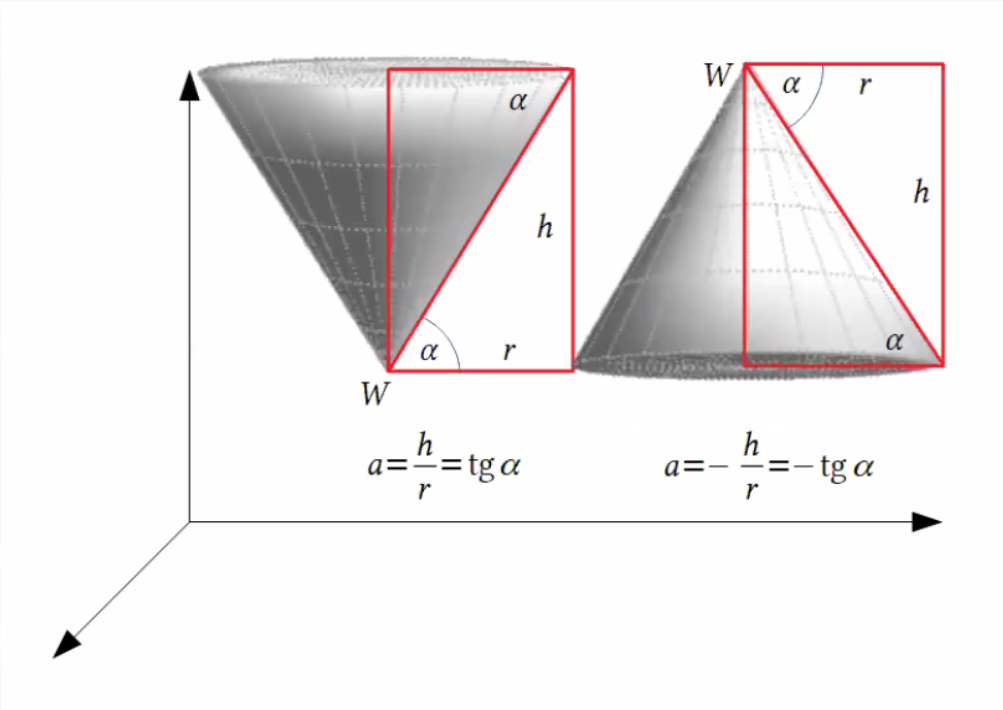
\includegraphics[scale=0.5]{img/stozek_wlzm.png}
\end{itemize}

Powierzchnia stożkowa i półsfera są szczególnymi przypadkami tzw. \underline{powierzchni obrotowych} w $\mathbb{R}^3$. \\

Powierzchnią obrotową w $\mathbb{R}^3$ wokół osi $Z$ będziemy nazywali zbiór wszystkich możliwych punktów
$(x,y,z)$ taki, że podstawienie $r = \sqrt{x^2 + y^2}$ wyznacza zbiór $z$ jako współrzędne wszystkich par $(z,r)$
tworzących pewną krzywą na płaszczyźnie, przy czym zbiór wszystkich $r \geq 0$ jest zbiorem otwartym.

Zatem jeżeli ta powierzchnia jest dana przez pewne równanie postaci
$$ F(x,y,z) = 0 $$
to podstawienie $ r = \sqrt{x^2 + y^2} $ usuwa wszystkie $x$ i $y$ i prowadzi do równania zależnego tylko od $z$ oraz $r$.

W szczególności gdy mamy $z = f(x,y)$ i podstawienie $r$ powoduje, że $f$ zależy tylko od $r$ to wykresem $f$ jest powierzchnia
obrotowa wokół osi $Z$. \\

\begin{tw}{Geometryczne własności takiej powierzchni}

\begin{itemize}
    \item Niepuste przecięcie powierzchni z dowolną płaszczyzną prostopadłą do osi $Z$ jest punktem, okręgiem lub sumą tych zbiorów.
    \item Niepuste przecięcie powierzchni z dowolną płaszczyzną zawierającą oś $Z$ jest krzywą o tym samym kształcie. \\
\end{itemize}

\end{tw}

Na przykład dla powierzchni stożkowej $ z = a\sqrt{x^2 + y^2}, \ a > 0 $, przecięcie płaszczyzną prostopadłą do osi $Z$ jest okręgiem
lub wierzchołkiem, a przecięcie płaszczyzną zawierającą oś $Z$ jest sumą dwóch półprostych wychodzących z wierzchołka.

\begin{center}
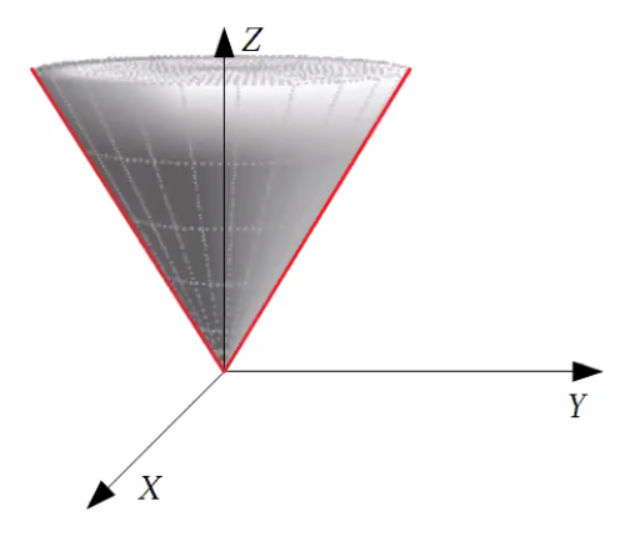
\includegraphics[scale=0.6]{img/stozek_wlzm_2.png}
\end{center}

Sposób rysowania takich powierzchni opiera się na spotstrzeżeniu, że dla $x = 0$ i $y \geq 0$ mamy $ r = \sqrt{y^2} = y \geq 0 $.
Zatem rysujemy w płaszczyźnie $YZ$ wykres odpowiedniej krzywej dla $y \geq 0$, a następnie obracamy go wokół osi $Z$. Tworzy to
żądaną powierzchnię obrotową. \\

Poprzedni przykład raz jeszcze: $ z = a\sqrt{x^2 + y^2}, \ a > 0 $.

Tutaj dla $ r = \sqrt{x^2 + y^2} \geq 0 $ mamy $z =ar$. Zatem biorąc $ r = y \geq 0 $ w płaszczyźnie $YZ$ dostajemy wykres
funkcji liniowej $ z = f(0, y) = ay, \ y \geq 0 $. Jest to półprosta

\begin{center}
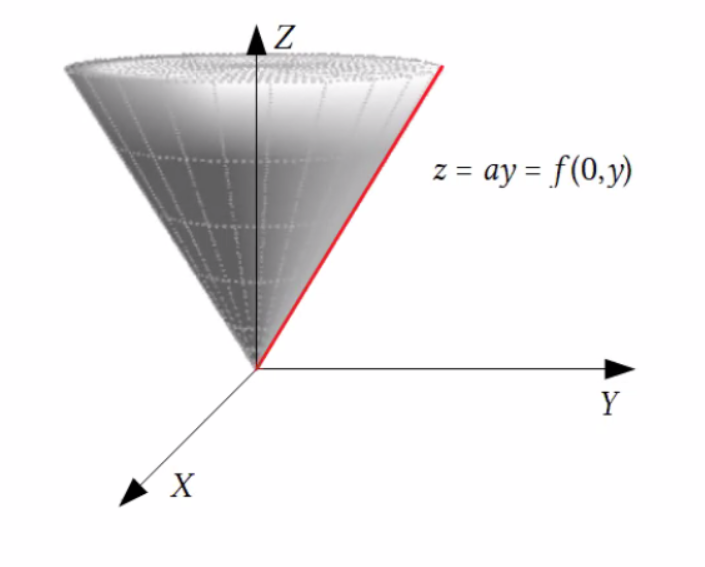
\includegraphics[scale=0.6]{img/stozek_wlzm_3.png}
\end{center}

Rozszerzanie powyższego przypadku -- powierzchnia obrotowa wokół osi równoległej do osi $Z$.

Jeżeli dla pewnych $x_0, y_0 \in \mathbb{R}$ podstawienie $ r = \sqrt{(x - x_0)^2 + (y - y_0)^2} $ usuwa wszystkie $x$ i $y$ i prowadzi
do równania zależnego tylko od $z$ oraz $r$ to dana powierzchnia jest powierzchnią obrotową wokół prostej
$ L : x = x_0, \ y = y_0, \ z\in \mathbb{R} $.

Jest to zatem przypadek powierczhni opisanej poprzednio (czyli dla $x_0 = y_0 = 0$) ale przesunięty następnie o wektor $ \vec{v} = [x_0, y_0, 0] $. \\

\begin{przyklad}
Powierzchnia dana równaniem $ z = (x+2)^2 + (y-1)^2 $
Tutaj mamy $ x_0 = -2 $ oraz $ y_0 = 1 $ i podstawienie $ r = \sqrt{(x+2)^2 + (y-1)^2} $ daje równanie $ z = r^2, \ r \geq 0 $.
Zatem biorąc $ r = y \geq 0 $ w płaszczyźnie $YZ$ dostajemy wykres funkcji $ z = f(0, y) = y^2, \ y \geq 0 $. Jest to prawa gałąź
paraboli.

Obracając ją następnie wokół osi $Z$ dostajemy powierzchnię zwaną paraboloidą.

\begin{center}
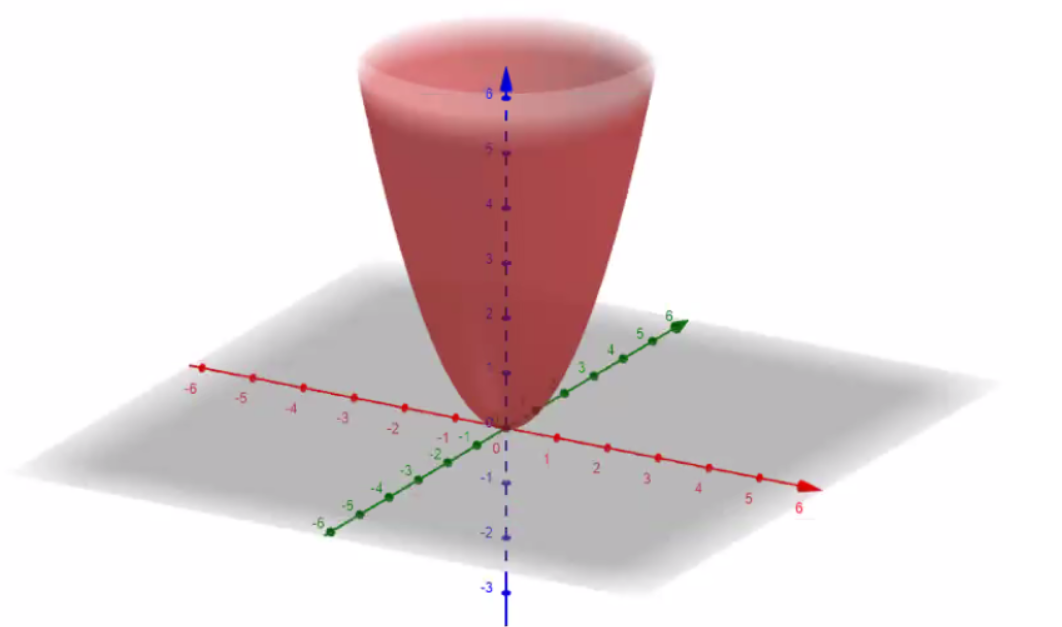
\includegraphics[scale=0.6]{img/paraboloida.png}
\end{center}

Na koniec przesuwamy powyższą powierzchnię o wektor $ \vec{v} = [x_0, y_0, 0] = [-2, 1, 0] $ i to daje naszą powierzchnię.
\end{przyklad}

\subsection*{Inny typ powierzchni -- tzw. powierzchnie walcowe}
\addcontentsline{toc}{subsection}{Powierzchnie walcowe}

Powierzchnia jest nazywana powierzchnią walcową równoległą do osi $Z$ jeżeli z faktu, że punkt $ (x_0,y_0,z_0) $
należy do powierzchni wynika, że dla dowolnego $z$ każdy punkt postaci $(x_0, y_0, z_0)$ też należy do tej powierzchni.

To oznacza, że jeżeli taka powierzchnia jest dana przez pewne wyrażenie to równanie to \textbf{nie zawiera} zmiennej $z$.

Geometrycznie -- niepuste przecięcie powierzchni z dowolną płaszczyzną równoległą do osi $Z$ daje krzywą o tym samym kształcie.

Stąd sposób tworzenia wykresów takich powierzchni -- rysujemy w płaszczyźnie $XY$ (czyli dla $z=0$) krzywą zadaną wyjściową relacją,
a potem wykres tej krzywej przesuwamy wzdłuż osi $Z$ i to generuje daną powierzchnię. \\ 

Dwa pozostałe przypadki są analogiczne:

\begin{itemize}
    \item gdy relacja definiująca powierzchnię nie zawiera $x$ to rysujemy odpowiednią krzywą w płaszczyźnie $YZ$
    , a potem jej wykres przesuwamy wzdłuż osi $X$,
    \item gdy relacja definiująca powierzchnię nie zawiera $y$ to rysujemy odpowiednią krzywą w płaszczyźnie $XZ$,
    a potem jej wykres przesuwamy wzdłuż osi $Y$.
\end{itemize}

Stąd prosta reguła -- odpowiednią krzywą przesuwamy zawsze wzdłuż tej osi, która odpowiada zmiennej \textbf{nieobecnej} w równaniu. \\

\begin{przyklad}

Powierzchnia o równaniu $ x^2 + y^2 = 1 $.

Nie występuje $z$, a więc jest to powierzchnia walcowa równoległa do osi $Z$.

Wyznaczamy krzywą daną powyższą relacją w płaszczyźnie $XY$ -- jest to okrąg o środku w układzie współrzędnych i promieniu równym $1$.

Po przesunięciu tego okręgu wzdłuż osi $Z$ zostaje wygenerowana powierzchnia -- jest to powierzchnia boczna walca o nieskończonej długości.
Stąd bierze się nazwa tego typu krzywych.

\begin{center}
    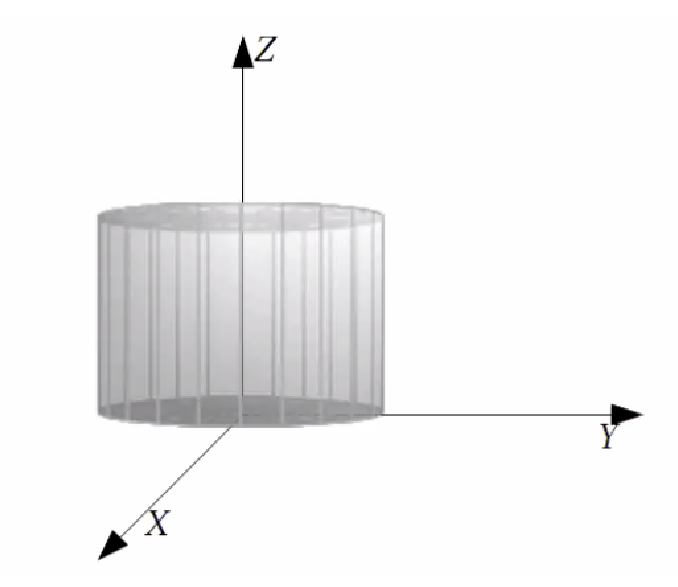
\includegraphics[scale=0.6]{img/walec.png}
\end{center}

\end{przyklad}


\begin{tw}{Definicja}

Poziomica funkcji $ z = f(x,y) $ na wysokości $h$ to zbiór
$$ D_h = \{ (x,y): f(x,y) = h \} $$
Jest to rzut na płaszczyznę $XY$ zbioru -- najczęściej krzywej -- będącego przekrojem wykresu $f$ płaszczyzną o równaniu $z = h$.
\end{tw}

\textbf{Interpretacja geograficzna}

Jeśli płaszczyzna $XY$ jest "mapą" i wyznacza "poziom morza", $z$ -- wysokością nad "poziomem morza", a wykres $f$ jest "rzeźbą terenu"
to poziomica jest krzywą na "mapie" która łączy punkty odpowiadające tej samej "wysokości" $h$.

Na podstawie zagęszczenia poziomic dla odpowiednio dobranych $h$ możemy przewidzieć kształt wykresu $f$ -- czy jest stromy czy płaski.


\subsection*{Pochodne cząstkowe pierwszego rzędu funkcji wielu zmiennych}
\addcontentsline{toc}{subsection}{Pochodne cząstkowe pierwszego rzędu funkcji wielu zmiennych}

Są to pochodne danej funkcji liczone względem jednej zmiennej, a pozostałe zmienne są stałe i przyjmują rolę parametrów.

Oznaczenie dla $ f = f(x,y) $:

$$ \dpartial{f}{x} \ \textrm{lub} \ f_x \ \textrm{-- pochodna po} \ x $$
$$ \dpartial{f}{y} \ \textrm{lub} \ f_y \ \textrm{-- pochodna po} \ y $$

Formalna definicja: 
$$ \dpartial{f}{x} (x_0,y_0) = \lim_{h \to 0} \frac{f(x_0 + h, y_0) - \fzero}{h} $$

$$ \dpartial{f}{y} (x_0,y_0) = \lim_{h \to 0} \frac{f(x_0, y_0 + h) - \fzero}{h} $$

Dla funkcji $n$ zmiennych $ f = f(x_1, x_2, ..., x_n) $:
$$ \dpartial{f}{x_i} (x_1, x_2, ..., x_n) = \lim_{h \to 0} \frac{f(x_1, x_2, ..., x_{i - 1}, 
\textcolor{blue}{x_i + h}, x_{i + 1}, ..., x_n) - f(x_1, x_2, ..., \textcolor{blue}{x_i}, ..., x_n)}{h} $$ \\


\subsection*{Interpretacja geometryczna dla funkcji 2 zmiennych}
\addcontentsline{toc}{subsection}{Interpretacja geometryczna dla funkcji 2 zmiennych}

Wykres każdej funkcji $f$ dwóch zmiennych można przeciąć płaszczyzną równoległą do osi $Z$. Powstaje wtedy pewna krzywa, która jest częścią wspólną wykresu $f$
oraz płaszczyzny. Jest to szczególny przypadek tzw. funkcji \underline{warunkowej} o której wkrótce powiemy więcej. \\

Gdy taka krzywa jest regularna to możemy liczyć dla niej pochodną.

Gdy płaszczyzna przekroju przechodzi przez punkt $ P=(x_0, y_0, \fzero) $ to pochodna tej krzywej jest równa

\begin{itemize}
    \item $ \dpartial{f}{x} (x_0, y_0) $, gdy płaszczyzna jest $\parallel XZ $,
    \item $ \dpartial{f}{y} (x_0, y_0) $, gdy płaszczyzna jest $\parallel YZ $. 
\end{itemize}

\begin{center}
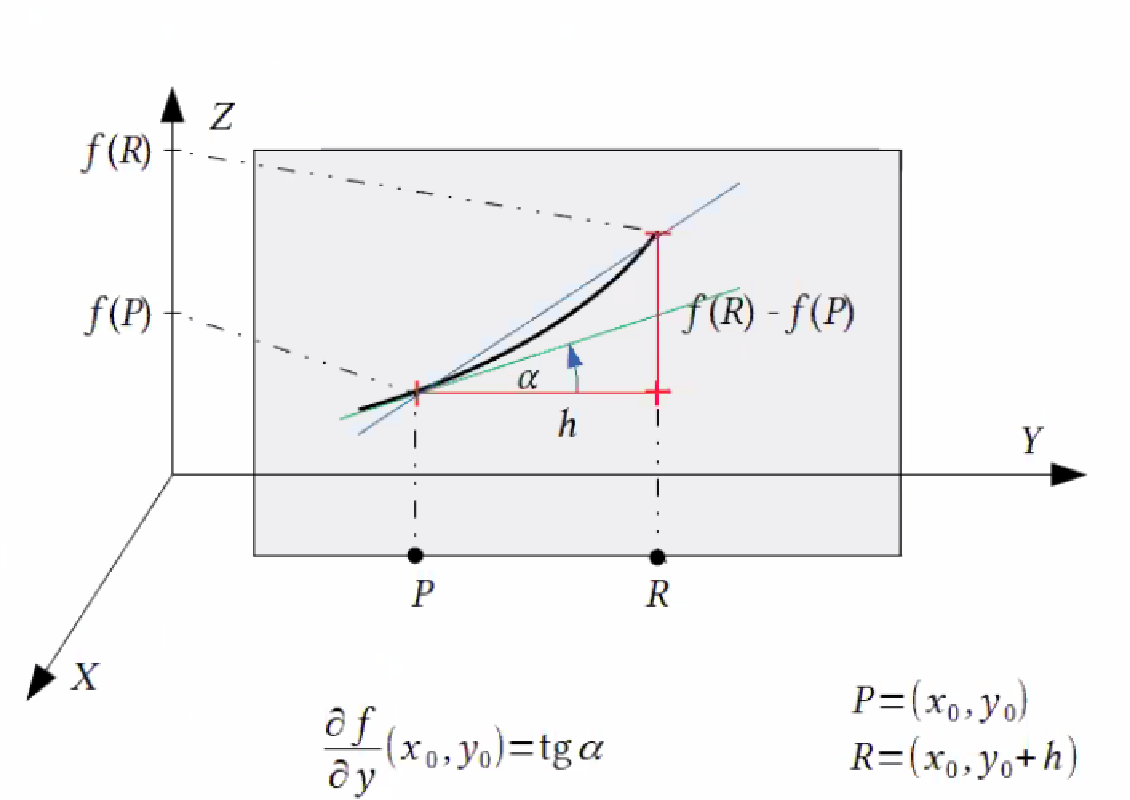
\includegraphics[scale=0.4]{img/interpretacja_geom.png}
\end{center}

\textbf{Sposób wyznaczania pochodnych cząstkowych w praktyce}

Ponieważ tylko jedna zmienna jest w użyciu, a pozostałe stają się parametrami to korzystamy z reguł różniczkowania
funkcji $1$ zmiennej.

Pamiętać należy, że dla wybranej zmiennej dowolne wyrażenie z każdą inną zmienną \textbf{staje się stałą} i jej pochodna
po wybranej zmiennej jest \textbf{równa 0}.

\begin{przyklad}
\[ \dpartial{}{y} (4x^2 + 3 \sin x + 5) = 0, \quad \dpartial{}{x} (ye^{z + 2y}) = 0 \quad \textrm{itd.} \]
\end{przyklad}

\begin{przyklad}

$$ f(x,y) = x \sin (xy^3) $$
Wtedy różniczkując po $x$ mamy pochodną iloczynu:
\[ \dpartial{f}{x} = f_x = (x)_x \cdot \sin(xy^3) + x \cdot (\sin (xy^3))_x = \sin(xy^3) + x \cdot \cos(xy^3) \cdot y^3 \]

Natomiast różniczkując po $y$ mamy mnożenie $\sin (xy^3)$ przez stałą dla $y$ (czyli $x$) i nie trzeba stosować pochodnej iloczynu
\[ \dpartial{f}{y} = f_y = (x \cdot \sin (xy^3))_y = x \cdot (\sin (xy^3))_y = x \cdot \cos(xy^3) \cdot 3y^2x \]
\end{przyklad}


\subsection*{Pochodne drugiego rzędu}
\addcontentsline{toc}{subsection}{Pochodne drugiego rzędu}

Mając pochodne $1$ rzędu definiujemy pochodne drugiego rzędu jako pochodne pierwszego rzędu z pochodnych pierwszego rzędu.
W szczególności, dla $ f = f(x,y) $ mamy $4$ pochodne drugiego rzędu. \\

Pochodne \underline{jednorodne} po danej zmiennej:
\begin{itemize}
    \item $ \frac{\partial^2 f}{\partial x^2} = \dpartial{}{x} \left( \dpartial{f}{x} \right) $ -- dwukrotne różniczkowanie $f$ po $x$,
    \item $ \frac{\partial^2 f}{\partial y^2} = \dpartial{}{y} \left( \dpartial{f}{y} \right) $ -- dwukrotne różniczkowanie $f$ po $y$,
\end{itemize}

Pochodne \underline{mieszane}:

\begin{itemize}
    \item $ \frac{\partial^2 f}{\partial y \partial x} = \dpartial{}{y} \left( \dpartial{f}{x} \right) $ -- różniczkowanie wpierw po $x$, potem po $y$,
    \item $ \frac{\partial^2 f}{\partial x \partial y} = \dpartial{}{x} \left( \dpartial{f}{y} \right) $ -- różniczkowanie wpierw po $y$, potem po $x$, \\
\end{itemize}

Inne oznaczenia to $ f_{xx}, f_{yy}, f_{xy}, f_{yx} $, gdzie indeks dolny oznacza zmienne, po których kolejno różniczkujemy.

W przypadku pochodnych mieszanych $ f_{xy}, f_{yx} $, trzeba ustalić kolejność różniczkowania.

Przyjmujemy naturalną kolejność, wtedy mamy $ f_{xy} = (f_x)_y $ \ oraz \ $ f_{yx} = (f_y)_x $,

co oznacza, że 

$ \frac{\partial^2 f}{\partial y \partial x} = f_{xy} $ \ i \ $ \frac{\partial^2 f}{\partial x \partial y} = f_{yx} $. \\

Dla funkcji $n$ zmiennych $ f = f(x_1, x_2, ..., x_n) $:
$$ \frac{\partial^2 f}{\partial x_j \partial x_i} = \dpartial{}{x_j} \left( \dpartial{f}{x_i} \right) = (f_{x_i})_{x_j} = f_{x_i x_j} $$ \\

\begin{przyklad}

$$ f(x,y) = \frac{2^y}{x+1} $$

$$ \textrm{Tutaj} \quad  f_x = -\frac{2^y}{(x+1)^2}, \ f_y = \frac{2^y \ln 2}{x+1} \quad \textrm{oraz} $$

$$ f_{xx} = (f_x)_x = \left( - \frac{2^y}{(x+1)^2} \right)_x = -2^y \left( \frac{1}{(x+1)^2} \right)_x = 2^y \cdot \frac{2}{(x+1)^3} $$

$$ f_{yy} = (f_y)_y = \left( \frac{2^y \ln 2}{x+1} \right)_y = \frac{\ln2}{x+1} \cdot (2^y)_y = \frac{2^y \cdot (\ln2)^2}{x+1} $$

$$ f_{xy} = (f_x)_y = \left( - \frac{2^y}{(x+1)^2} \right)_y = \left( \frac{-1}{(x+1)^2} \right) \cdot (2^y)_y = - \frac{2^y \ln2}{(x+1)^2} $$

$$ f_{yx} = (f_y)_x = \left( \frac{2^y \ln2}{x+1} \right)_x = 2^y \ln2 \left( \frac{1}{x+1} \right)_x = 2^y \ln2 \left( \frac{-1}{(x+1)^2} \right) = - \frac{2^y \ln2}{(x+1)^2} $$ \\

Otrzymaliśmy $ f_{xy} = f_{yx} $.

Jest to szczególny przypadek znanego twierdzenia.
\end{przyklad}

\begin{tw}{Twierdzenie Schwarza o pochodnych mieszanych}

Gdy pochodne mieszane drugiego rzędu są funkcjami ciągłymi w danym punkcie to są w tym punkcie równe.

W praktyce dla funkcji regularnych warunek ciągłości drugiego rzędu występuje zawsze na całych dziedzinach
stąd prawie zawsze zobaczymy równość wzorów pochodnych mieszanych.
\end{tw}

\begin{tw}{Definicja}
Niech $k \in \mathbb{N}^+$ \ oraz \ $ f = f(x_1, x_2, ..., x_n) $. Pochodna rzędu $k$ funkcji $f$ to funkcja
\[ \frac{\partial^k f}{\partial x_{n_1}... \partial x_{n_2} \partial x_{n_k}} = \dpartial{}{x_{n_k}}
= \left( ... \left( \dpartial{}{x_{n_2}} \left( \dpartial{f}{x_{n_1}} \right) \right) ... \right) = f_{x_{n_1}, x_{n_2}, ..., x_{n_k}} \]

gdzie zmienne \ $ x_{n_1}, x_{n_2}, ..., x_{n_k} $ są dowolnymi ze zmiennych \ $x_1, x_2, ..., x_n$. \bigskip

Oznacza to różniczkowanie funkcji $k$ razy, po kolei po zmiennych
\[ x_{n_1}, x_{n_2}, ..., x_{n_k} \]

\end{tw}

Pochodne jednorodne to te, w których różniczkujemy po tej samej zmiennej $k$ razy, np. $f_{xxx}$.

Pochodne mieszane to te pochodne, w których różniczkujemy przynajmniej po dwóch różnych zmiennych np. $ \frac{\partial^4 f}{\partial x \partial x \partial y \partial x} = f_{xyxx} $

Twierdzenie Schwarza pozostaje prawdziwe dla pochodnych mieszanych rzędu $k$.

\subsection*{Płaszczyzna styczna do funkcji dwóch zmiennych}
\addcontentsline{toc}{subsection}{Płaszczyzna styczna do funkcji dwóch zmiennych}

\begin{tw}{Definicja}
Niech \ $ R = (x,y,z) $ \ oraz \ $ P = (x_0, y_0, z_0) $. Definiujemy zbieżność
\[ R \to P \ \Leftrightarrow \ x \to x_0 \ \land \ y \to y_0 \ \land \ z \to z_0 \]
Nazywamy to zbieżnością po współrzędnych.

\end{tw}

\begin{tw}{Definicja}

Niech teraz $P$ i $R$ należą do wykresu funkcji $f$. 

Czyli 
\[ z = f(x,y), \quad z_0 = \fzero \]
Ponadto niech $ \Pi $ będzie płaszczyzną przechodzącą przez $P$.

$\Pi$ nazywamy \underline{płaszczyzną styczną} do wykresu $f$ w punkcie $P$ jeżeli kąt między prostą $PR$ oraz płaszczyzną $\Pi$ dąży do 0, gdy $R \to P$.

Jest to uogólnienie prostej stycznej do wykresu funkcji jednej zmiennej.
\end{tw}

\begin{tw}{Definicja}
$ f = f(x,y) $ jest funkcją \underline{różniczkowalną} w punkcie \ $(x_0, y_0) \in D_f$, \ gdy istnieje płaszczyzna styczna do wykresu $f$
w punkcie \ $ P = (x_0, y_0, \fzero) $.
\end{tw}

Przykład funkcji nieróżniczkowalnej w pewnym punkcie: powierzchnia stożkowa w wierzchołku (zobacz rysunek powierzchni stożkowych str. 50)

\begin{tw}{Twierdzenie}
Gdy na pewnym kole bez brzegu zawierającym \ $(x_0, y_0) \in D_f $ \ $f$ ma ciągłe pochodne cząstkowe pierwszego rzędu to $f$ jest różniczkowalna w punkcie $(x_0, y_0)$.
\end{tw}

\begin{tw}{Twierdzenie -- wzór na płaszczyznę styczną do $f$}
    Jeżeli $f$ jest różniczkowalna w punkcie $(x_0, y_0)$ to płaszczyzna styczna do wykresu $f$ w $P = (x_0, y_0, \fzero)$ jest dana wzorem
    \[ z - \fzero = f_x(x_0, y_0) \cdot (x - x_0) + f_y(x_0, y_0) \cdot (y - y_0) \]
\end{tw}

Uwagi 
\begin{itemize}
    \item Warunek ciągłości pochodnych na kole jest spełniony dla zdecydowanej większości funkcji elemetnarnych na całej dziedzinie funkcji.
    \item Wzór na płaszczyznę styczną jest analogiczny do wzoru na prostą styczną do funkcji jednej zmiennej.
    \item Płaszczyznę styczną można zapisać w postaci ogólnej
    \[ A(x - x_0) + B(y - y_0) - 1(z - z_0) = 0 \]
    gdzie
    \[ z_0 = \fzero, \quad A = f_x(x_0, y_0), \quad B = f_y(x_0, y_0) \]
    Stąd wektorem normalnym jest
    \[ \vec{n} = [A, B, -1] = [f_x(x_0, y_0), f_y(x_0, y_0), -1] \] 
\end{itemize}

\begin{przykladbig}
    Dana jest funkcja \ $ f(x,y) = x^2 - 2y^2 $

    a) Znaleźć płaszczyznę styczną do wykresu $f$ w punkcie \ $ P = (1, 2, z_0) $.

    b) Znaleźć wszystkie punkty wykresu $f$ w których płaszczyzna styczna jest równoległa do płaszczyzny \ $ \Pi_1: x - 2y + 2z + 5 = 0 $
    \bigskip

    a) $ \Pi_s $ w $ P = (1, 2, z_0)$

    $ z_0 = f(1,2) = -7 $

    \[ \begin{array}{cc}
        f_x = 2x & A = f_x(1,2) = 2 \\
        f_y = -4y & B = f_y(1,2) = -8
    \end{array} \]

    Wzór 
    \[ z - (-7) = 2(x-1) - 8(x-2) \quad \text{lub} \quad \ 2(x-1) - 8(y-2) - (z+7) = 0 \]

    b)
    \[ \Pi_s \ \| \ \Pi : x - 2y + 2z + 5 = 0 \]
    \[ \vec{n} = [-1,-2,2] \ \bot \ \Pi \]
    \[ \vec{n_s} = [f_x, f_y, -1] \ \bot \ \Pi_s \]

    \[ \Pi \ \| \ \Pi_s \ \Leftrightarrow \ \vec{n} \ \| \ \vec{n_s} \ \Leftrightarrow \ \frac{f_x}{1} = \frac{f_y}{-2} = \frac{-1}{2} \]

    Trzeba zatem rozwiązać układ równań
    \[ \begin{cases}
        f_x = -\frac{1}{2} = 2x \\
        f_y = 1 = -4y
    \end{cases} \]

    Rozwiązanie to
    \[ x = x_0 = -\frac{1}{4} \]
    \[ y = y_0 = -\frac{1}{4} \]

    Stąd
    \[ z_0 = f(-\frac{1}{4}, -\frac{1}{4}) = -\frac{1}{16} \]
    I punkt to jest
    \[ P = (-\frac{1}{4}, -\frac{1}{4}, -\frac{1}{16}) \]
\end{przykladbig}

Bezpośrednie zastosowanie: \underline{przybliżanie funkcji płaszczyzą styczną}

Równanie płaszczyzny stycznej $\Pi$ do wykresu $f$ w $P = (x_0, y_0, \fzero)$ można zapisać wzorem

\[ z = \fzero + f_x(x_0, y_0) \cdot (x - x_0) + f_y(x_0, y_0) \cdot (y - y_0) \]

Gdy teraz \ $ R = (x, y, f(x,y)), \ Q = (x,y,z) \in \Pi $ \ i \ $ x \approx x_0 $ oraz \ $ y \approx y_0 $ to 
\ $ R \approx P \approx Q $, \ a więc \ $ R \approx Q $ \ i \ $ z \approx f(x,y) $.

To daje wzór na przybliżoną wartość \ $f(x,y)$:

\[ f(x,y) \approx f(x_0,y_0) + f_x(x_0, y_0) \cdot (x - x_0 ) + f_y(x_0, y_0) \cdot (y - y_0) \]

Zastosowanie:
\begin{itemize}
    \item $ x_0, y_0 $ -- "ładne": łatwe do obliczenia,
    \item $ x,y $ -- to co mamy w zadaniu.
\end{itemize}

\begin{przyklad}
    Obliczyć w przybliżeniu i bez kalkulatora $ (2,005)^5 \ln(0,98) $ \medskip

    Mamy \ $ (2,005)^5 \ln(0,98) = f(2.005, 0.98) $.

    Zatem
    \[ f(x,y) = x^5 \ln y, \ x = 2,005, \ y = 0,98 \]

    Bierzemy \ $x_0 = 2$ \ oraz \ $ y_0 = 1 $.

    To daje
    \[ f_x = 5x^4 \ln y, \quad f_y = \frac{x^5}{y}, \quad f_x(2,1) = 0, \quad f_y(2,1) = 32 \quad \text{oraz} \quad f(2,1) = 0 \]

    Zatem
    \[ (2,005)^5 \ln (0,98) \approx 0 + 0 \cdot (2,005 - 2) + 32 \cdot(0,98 - 1) = -0,64 \]

    Dokładna wartość: $ -0,65461 $. Błąd wynosi ok. 0,015 czyli 2,34\%.
\end{przyklad}

Dalsze zastosowanie wzoru

Biorąc \ $ x - x_0 = \Delta x, \quad y - y_0 = \Delta y $ \ mamy \ $ x = \Delta x + x_0, \quad y = \Delta y + y_0 $.
\medskip

To daje wzór
\[ f(x_0 + \Delta x, y_0 + \Delta y) \approx \fzero + f_x(x_0, y_0) \cdot \Delta x + f_y(x_0, y_0) \cdot \Delta y \]
Czyli
\[ f(x_0 + \Delta x, y_0 + \Delta y) - \fzero \approx f_x(x_0, y_0) \cdot \Delta x + f_y(x_0, y_0) \cdot \Delta y \]

Oznaczając przez $ \Delta f $ "błąd bezwzględny funkcji" mamy
\[ \Delta f  = | f(x_0 + \Delta x ,y_0 + \Delta y) - \fzero | \ \approx f_x(x_0, y_0) \cdot \Delta x + f_y(x_0, y_0) \cdot \Delta y \]

Gdy oba iloczyny pod modułem z prawej strony mają ten sam znak błędy kumulują się i mamy
\[ \Delta f \approx | f_x(x_0, y_0) | \ \cdot \ | \Delta x | \ + \ | f_y(x_0, y_0) | \ \cdot \ | \Delta y | \]

To jest wzór na tzw. \underline{różniczkę zupełną}.

Jest to uogólnienie wzoru z AM1 dla funkcji jednej zmiennej \ $ f = f(x) $:
\[ \Delta f \approx | f'(x_0) | \ \cdot \ | \Delta x | \]

Zastosowania -- przy pomiarach z błędem

Mierzymy $x$ z dokładnością $ | \Delta x| \approx 0 $.

Wówczas błąd bezwzględny pomiaru $f$ wynosi w przybliżeniu $ \Delta f $.

\begin{przyklad}
    W obwodzie zmierzono wartość prądu stałego \ $ I = 3 \ A \pm 0,1 \ A $ oraz rezystancję \ $ R = 2 \ \Omega \pm 0,01 \Omega $.

    Z jaką w przybliżeniu dokładnością zmierzymy wydzieloną moc? \bigskip

    Mamy
    \[ P = P(I, R) = I^2 R, \quad I_0 = 3, \quad R_0 = 2, \quad, \Delta I = \pm 0,1, \quad \Delta R = \pm 0,01 \]

    Czyli
    \[ P_I = 2 IR, \quad P_R = I^2, \quad P_I(3,2) = 12, \quad P_R(3,2) = 9 \]
    A więc
    \[ \Delta P = |12| \ \cdot 0,1 + |9| \ \cdot 0,01 = 1,29 [\textrm{W}] \]
\end{przyklad}


\subsection*{Pochodna kierunkowa}
\addcontentsline{toc}{subsection}{Pochodna kierunkowa}

\begin{tw}{Definicja}
    Dla funkcji 2 zmiennych \ $ f = f(x,y) $ \ pochodna ta mierzy zmienność $f$ w zadanym kierunku \ $ \vec{v} = [a,b] $.

    Geometrycznie, jest to wersja pochodnej jednostronnej krzywej, która jest częścią wspólną wykresu $f$ oraz płaszczyzny równoległej
    do osi $Z$ i do wektora $\vec{v}$.

    Oznaczenie :
    \[ \dpartial{f}{\vec{v}}(x,y) \quad \text{lub} \quad f_{\vec{v}}(x,y) \]
\end{tw}

\textbf{Uwaga! Do definicji będziemy zawsze używać wektorów jednostkowych:}
\[ |\vec{v}| = 1 \]

\begin{tw}{Ogólna definicja dla funkcji $n$ zmiennych}
    Ustalamy punkt $P$ w $\mathbb{R}^n$ i rozpatrujemy półprostą o początku w $P$ i o kierunku zgodnym z $\vec{v}$ czyli zbiór tych punktów
    $R$ dla których $\overrightarrow{PR}$ i $\vec{v}$ mają zgodne kierunki.

    Badamy proporcję różnicy wartości $f$ w punktach $R$ i $P$ do odległości $R$ od $P$ przy przejściu granicznym $ R \to P $.

    Daje to definicję
    \[ \dpartial{f}{\vec{v}}(P) = \lim_{R \to P} \frac{f(R) - f(P)}{|\overrightarrow{PR}|} \]

    \begin{center}
        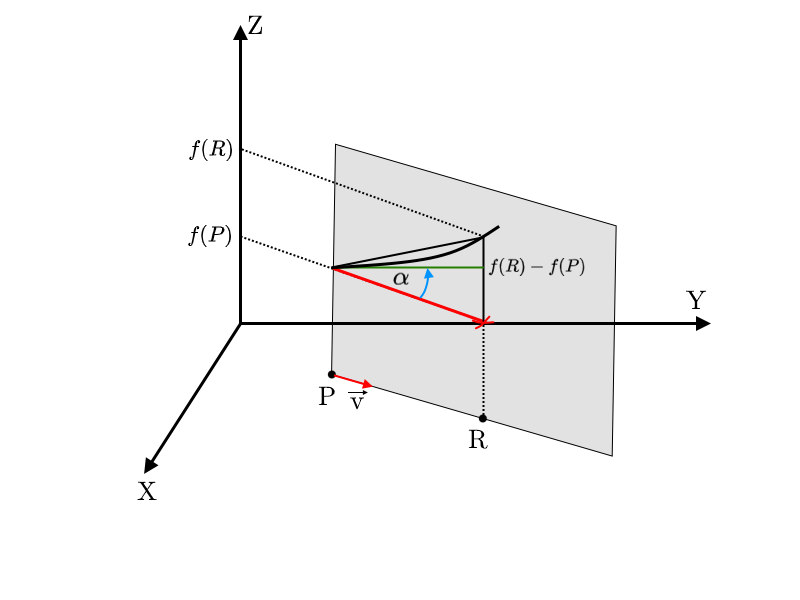
\includegraphics[scale=0.5]{img/pochodnakierunkowa.png}
    \end{center}
    \[ \dpartial{f}{\vec{v}}(P) = \tan \alpha \]
\end{tw}

W przypadku funkcji 2 zmiennych dla \ $ P = (x_0, y_0) $ \ i \ $ \vec{v} = [a,b] $ \ równanie parametryczne powyższej półprostej ma postać
\[ \begin{cases} 
    x = x_0 + at \\
    y = y_0 + bt
\end{cases} \quad \text{dla} \ t > 0 \]

To oznacza, że
\[ R = (x,y) = (x_0 + at, y_0 + bt) \quad \text{oraz} \quad \overrightarrow{PR} = t \cdot \vec{v} \]
A stąd
\[ |\overrightarrow{PR}| = |t \cdot \vec{v}| = |t| \cdot |\vec{v}| = t \cdot 1 = t \]

Ponieważ \ $ R \to P \ \Leftrightarrow \ t \to 0^+ $ \ oznacza, że
\[ \lim_{R \to P} \frac{f(R) - f(P)}{|\overrightarrow{PR}|} = \lim_{t \to 0^+} \frac{f(x_0 + at, y_0 + bt) - \fzero}{t} \]
a to daje równoważną definicję pochodnej kierunkowej:
\[ \dpartial{f}{\vec{v}} (x_0, y_0) = \lim_{t \to 0^+} \frac{f(x_0 + at, y_0 + bt) - \fzero}{t}, \quad \text{gdzie} \ \vec{v} = [a,b], \ |\vec{v}| = 1 \]

\begin{przyklad}
    \[ \dpartial{f}{\vec{v}} (0,1) = \lim_{t \to 0^+} \frac{f \left( 0 - \frac{\sqrt{2}}{2}t, 1 + \frac{\sqrt{2}}{2}t \right) - f(0,1)}{t}
    = \lim_{t \to 0^+} \frac{ \left| -\frac{\sqrt{2}}{2}t \right| + 3 \left| 1 + \frac{\sqrt{2}}{2}t \right| - 3 }{t} = \]
    \[ \lim_{t \to 0^+} \frac{ \frac{\sqrt{2}}{2}t + 3 \left( 1 + \frac{\sqrt{2}}{2}t \right) - 3 }{t} = \lim_{t \to 0^+} \frac{4 \cdot \frac{\sqrt{2}}{2}t}{t} = 2 \sqrt{2} \]
\end{przyklad}

Z definicji liczymy tylko dla funkcji mało regularnych. Gdy pochodne cząstkowe $f$ są ciągle to mamy lepszy wzór z użyciem \underline{gradientu}.

\subsection*{Gradient}
\addcontentsline{toc}{subsection}{Gradient}

\begin{tw}{Definicja}
    Gradient funkcji w danym punkcie -- wektor pochodnych cząstkowych pierwszego rzędu funkcji $f$ w danym punkcie.

    Oznaczenie: $ \text{grad}\, f$ \ lub \ $ \nabla f $.

    Dla funkcji 2 zmiennych i punktu $ P = (x_0, y_0) $
    \[ \text{grad}\, \fzero = [f_x(x_0, y_0), f_y(x_0, y_0)] \]

    Dla funkcji $n$ zmiennych \ $ f = f(x_1, x_2, ..., x_n) $ \ i punktu \ $ P = (a_1, a_2, ..., a_n) \in \mathbb{R}^n $
    \[ \text{grad} \, f(P) = [f_{x_1}(P), f_{x_2}(P), ..., f_{x_n}(P)] \]
\end{tw}

\begin{tw}{Twierdzenie}
    Gdy pochodne cząstkowe $f$ są ciągłe w \ $ (x_0, y_0) $ \ i \ $ \vec{v} = [a,b] $ \ oraz \ $ |\vec{v}| = 1 $ \ to
    \[ \dpartial{f}{\vec{v}} (x_0, y_0) = \vec{v} \circ (\text{grad} \, \fzero) = a \cdot f_x(x_0, y_0) + b \cdot f_y(x_0, y_0) \]
    Wzór rozszerza się do funkcji większej ilości zmiennych.    
\end{tw}

\begin{przyklad}
    \[ f(x,y) = x^2 \cdot y^3, \quad \vec{v} =\left[ -\frac{1}{2}, \frac{\sqrt{3}}{2} \right] \]
    Obliczyć $ f_{\vec{v}} (-1, 1) $. \bigskip

    Mamy
    \[ f_x = 2xy^3, \quad f_y = 3x^2 y^2 \]
    \[ f_x(-1, 1) = -2, \quad f_y(-1, 1) = 3, \quad \text{grad}\, f(-1, 1) = [-2, 3] \]
    \[ f_{\vec{v}} = [-2, 3] \circ \left[ -\frac{1}{2}, \frac{\sqrt{3}}{2} \right] = 1 + \frac{3 \sqrt{3}}{2} \]
\end{przyklad}

Dalej,
\[ \vec{v} \circ \text{grad}\, \fzero = 1 \cdot | \text{grad}\ \fzero | \cdot \cos \alpha \]
gdzie $\alpha$ jest kątem między tymi dwoma wektorami.

To daje następujące wnioski:

\begin{tw}{Twierdzenie}
    Gdy \ $ \text{grad} \, \fzero = \vec{0} $
    \quad to \quad
    $ \dpartial{f}{\vec{v}} (x_0, y_0) = 0 $
    \quad dla dowolnego $ \vec{v} $.
\end{tw}

\begin{tw}{Twierdzenie}
    $ \dpartial{f}{\vec{v}} (x_0, y_0) $ ma wartość największą kiedy $\vec{v}$ i grad $\ \fzero $ mają zgodne kierunki.

    Ta największa wartość to \ $ | \text{grad}\, \fzero | $.
\end{tw}

\begin{tw}{Twierdzenie}
    $ \dpartial{f}{\vec{v}} (x_0, y_0) $ ma wartość najmniejszą kiedy $\vec{v}$ i grad $\ \fzero $ mają przeciwne kierunki.

    Ta najmniejsza wartość to \ $ -| \text{grad}\, \fzero | $.
\end{tw}

\begin{tw}{Twierdzenie}
    $ \dpartial{f}{\vec{v}} (x_0, y_0) = 0 $ \quad dla \quad $ \text{grad} \, \fzero \neq \vec{0} $
    \quad kiedy \quad
    $ \text{grad} \, \fzero \perp \vec{v} $
\end{tw}

\begin{tw}{Twierdzenie}
    Zbiór wartości \ $ \dpartial{f}{\vec{v}} (x_0, y_0) $ \ w zależności od $\vec{v}$ to przedział
    \[ [ -|\text{grad} \, \fzero|, |\text{grad} \, \fzero | ] \]
    Skrajne wartości są osiągane dla dokładnie jednego wektora (zob. punkty 2 i 3), a pozostałe -- dla dokładnie dwóch wektorów $\vec{v}$.
\end{tw}

\begin{przyklad}
    Dana jest funkcja \ \[ f(x,y) = (x^2 + y^2)e^{x-y} \]

    1.Znaleźć wszystkie wersory $\vec{v}$ dla których \ $ f_{\vec{v}} (-1, 1) $
    
    a) jest największa

    b) jest najmniejsza \medskip

    2. Wyznaczyć zbiór wszystkich punktów (x,y) dla których pochodna kierunkowa w kierunku wersora \ $ \vec{v} = \left[ \frac{3}{5}, \frac{4}{5} \right] $ \ jest równa 0.
    \bigskip

    Wprowadzić wektor $ \vec{v} = [a,b] $ \ co daje
    \[ f_{\vec{v}} (-1, 1) = [a,b] \circ [3e^{-3}, -e^{-3}] = 3e^{-3} a - e^{-3}b \]
    Następnie trzeba analizować tę funkcję \textbf{nie zapominając o dodatkowym warunku}
    \[ \vec{v} = 1 \ \Leftrightarrow \ a^2 + b^2 = 1 \]
    Prowadzi to do układu równań, jest dłuższe i bardziej skomplikowane

    W części 2 potrzebna jest metoda analityczna.
    
    Korzystając ze wzoru na gradient z części a) Mamy
    \[ f_{\vec{v}} = (x,y) = grad\, f(x,y) \circ \vec{v} = [e^{x-y} (2x + x^2 + y^2), e^{x-y}(2y - x^2 - y^2)] \circ \left[ \frac{3}{5}, \frac{4}{5} \right] = \]
    \[ \frac{3}{5} e^{x-y} (2x + x^2 + y^2) + \frac{4}{5} e^{x-y} (2y - x^2 - y^2) = \frac{1}{5} e^{x-y} (6x + 8y - x^2 - y^2) = 0 \]

    To oznacza, że \ $ 6x + 8y - x^2 - y^2 = 0 $

    Jest to równanie okręgu -- po sprowadzeniu do postaci kanonicznej mamy \bigskip

    \textbf{Ciąg dalszy nastąpi po wykładzie w dniu 8.05.2023}
\end{przyklad}

\subsection*{Zbieżność w $\mathbb{R}^k$ i granice funkcji wielu zmiennych}
\addcontentsline{toc}{subsection}{Zbieżność w $R^k$  i granice funkcji wielu zmiennych}

Rozpatrujemy ciąg wielu punktów $ P_n = (x_n, y_n) \in \mathbb{R}^2 $.

Równoważnie możemy myśleć o wektorach $ \vec{v} \in \mathbb{R}^2 $ biorąc wektory pozycyjne punktów $P_n$ czyli $\vec{v} = \vec{OP}_n$.

Niech teraz $ P_0 = (x_0, y_0) \in \mathbb{R}^2 $. Mówimy, że $ P_n \to P_0 $, gdy odległość między $P_n$ i $P_0$ zbiega $0$.

Formalnie
$$ \limn P_n = P_0 \ \Leftrightarrow \ \limn |\overrightarrow{P_0 P_n}| = 0
\ \Leftrightarrow \ \limn \sqrt{(x_n - x_0)^2 + (y_n - y_0)^2} = 0 $$

Podobnie, gdy
$$ P_n = (x_n, y_n, z_n) \in \mathbb{R}^3 \quad \textrm{i} \quad P_0 = (x_0, y_0, z_0) \in \mathbb{R}^3 $$

To definiujemy
$$ \limn P_n = P_0 \ \Leftrightarrow \ \limn |\overrightarrow{P_0 P_n}| = 0
\ \Leftrightarrow \ \limn \sqrt{(x_n - x_0)^2 + (y_n - y_0)^2 + (z_n - z_0)^2} = 0 $$

Analogicznie rozszerzamy tę definicję na przypadek $k$ -- wymiarowy. \\

Poniższe twierdzenie pokazuje, że zbieżność $ P_n \to P_0 $ może być zdefiniowana w równoważny sposób. \\

\begin{tw}{Twierdzenie -- zbieżność po współrzędnych }

Gdy
\[ P_n = (x_n, y_n) \in \mathbb{R}^2 \quad \textrm{i} \quad P_0 = (x_0, y_0) \in \mathbb{R}^2 \]
to mamy równoważność
\[ \limn P_n = P_0 \ \Leftrightarrow \ \limn x_n = x_0 \ \land \ \limn y_n = y_0 \]
\end{tw}

Dowód 

Implikacja $ \Leftarrow $ wynika bezpośrednio z arytmetyki granic :

Jeżeli $ \limn x_n = x_0 \ \land \ \limn y_n = y_0 $ to
$$ \limn |\overrightarrow{P_0 P_n}| = \limn \sqrt{(x_n - x_0)^2 + (y_n - y_0)^2} = \sqrt{(x_n - x_0)^2 + (y_n - y_0)^2} = 0 $$

Zatem
$$ \limn P_n = P_0 $$ \\

Implikacja $ \Rightarrow $ wynika z kolei z twierdzenia o 3 funkcjach. 

Mamy bowiem
$$ 0 \leq |x_n - x_0| = \sqrt{(x_n - x_0)^2} \leq \sqrt{(x_n - x_0)^2 + (y_n - y_0)^2} = |\overrightarrow{P_0 P_n}| $$

Teraz, gdy $ \limn P_n = P_0 \quad \textrm{to} \quad \limn |\overrightarrow{P_0 P_n}| = 0 $
i z twierdzenia o 3 ciągach dostajemy $ \limn |x_n - x_0| = 0 $ a to daje
$ \limn (x_n - x_0) = 0 \ \Leftrightarrow \ \limn x_n = x_0 $

Analogicznie otrzymujemy $ \limn y_n = y_0 $ \\

Jak łatwo zauważyć, twierdzenie ma analogiczną postać w przypadku wyższych wymiarów. \\

\begin{tw}{Definicja -- granica funkcji dwóch zmiennych w punkcie}

$ \lim_{(x,y) \to (x_0,y_0)} f(x,y) = L \ \Leftrightarrow $ dla dowolnych ciągów punktów $ (x_n, y_n) \neq (x_0, y_0) $
i takich, że $ \limn (x_n, y_n) = (x_0, y_0) $ zachodzi równość $ \limn f(x_n, y_n) = L $. \\

Definicja jest analogiczna w przypadku funkcji większej ilości zmiennych.

Równoważny zapis tej granicy, zgodny ze znaczeniem twierdzenia o zbieżności po współrzędnych to
$$ \lim_{\substack{x \to x_0 \\ y \to y_0}} f(x,y) = L $$

Twierdzenie o granicach znane dla funkcji jednej zmiennej (arytmetyka granic, symbole nieoznaczone itd.) pozostają prawdziwe.
\end{tw}

Główny problem -- nie da się bezpośrednio zastosować niektórych popularnych technik, np. reguły de l'Hospitala.

\subsection*{Popularne techniki liczenia granic funkcji wielu zmiennych}
\addcontentsline{toc}{subsection}{Popularne techniki liczenia granic funkcji wielu zmiennych}

\begin{enumerate}
    \item Twierdzenie o 3 funkcjach. Jeżeli dla wszystkich punktów $ P \in \mathbb{R}^k $ z pewnego sąsiedztwa punktu
    $ P_0 \in \mathbb{R}^k $ zachodzi nierówność 
    $$ d(P) \leq f(P) \leq g(P) \quad \textrm{i} \quad \lim_{P \to P_0} d(P) = \lim_{P \to P_0} g(P) = L \quad \textrm{to} \quad \lim_{P \to P_0} f(P) = L $$

    \item Sprowadzenie granicy do przypadku jednej zmiennej.
    
    Jeżeli istnieje nowa zmienna $ t = t(P) $ takie, że $ f(P) = g(t) $ oraz 
    $ \lim_{P \to P_0} t = t_0 $ \ i \linebreak \ $ \lim_{t \to t_0} g(t) = L $ \ to \ $ \lim_{P \to P_0} f(P) = L $ 

    \item \textbf{COŚ O BRAKU GRANICY XD}
    $ \lim_{P \to P_0} f(P) $ nie istnieje
\end{enumerate}

Przypadek 3 jest szczególnie częsty, gdy pojawia się symbol nieoznaczony.

W przypadku funkcji dwóch zmiennych najczęściej wybiera się ciągi punktów $P_n$ i $Q_n$ z dwóch różnych krzywych.

$P$ jest wtedy z wykresu jakiejś krzywej: $ y=g(x)$ \ lub \ $x=g(y)$.

$Q$ jest z wykresu innej krzywej: $y=h(x)$ \ lub \ $x=h(y)$.

Obie krzywe muszą spotykać się w punkcie granicznym $P_0$.

Wtedy granice \ $ \lim_{P \to P_0} f(P) $ \quad i \quad $ \lim_{Q \to P_0} f(Q) $ \ stają się granicami funkcji jednej zmiennej. \\

\begin{przyklad}

$$ \lim_{\substack{x \to 0 \\ y \to 0}} (x^2 + 4y^2) \cos \left( x - 5y + \frac{2}{x} \right) $$

Wiemy, że \ $ x^2 + 4y^2 \geq 0 $ \ oraz \ $ -1 \leq \cos \left( x - 5y \frac{2}{x} \right) \leq 1 $, \ a stąd
$$ -(x^2 + 4y^2) \leq (x^2 + 4y^2) \cos \left( x - 5y + \frac{2}{x} \right) \leq x^2 + 4y^2 $$

Ponieważ 
$$ \lim_{\substack{x \to 0 \\ y \to 0}} (x^2 + 4y^2) = 0 = \lim_{\substack{x \to 0 \\ y \to 0}} (-(x^2 + 4y^2)) $$
z twiedzenia o 3 ciągach otrzymujemy
$$ \lim_{\substack{x \to 0 \\ y \to 0}} (x^2 + 4y^2) \cos \left( x - 5y + \frac{2}{x} \right) = 0 $$ \\

$$ \lim_{\substack{x \to 1 \\ y \to 1 \\ z \to 0}} \frac{2x - y + z - 1 - \ln(2x - y + z)}{(2x - y + z - 1)^2} $$

Tutaj możemy podstawić $ t = 2x - y + z $. Wtedy $ \lim_{\substack{x \to 1 \\ y \to 1 \\ z \to 0}} t = 1 $

i mamy

$$ \lim_{\substack{x \to 1 \\ y \to 1 \\ z \to 0}} \frac{2x - y + z - 1 - \ln(2x - y + z)}{(2x - y + z - 1)^2}
= \lim_{t \to 1} \frac{t - 1 - \ln t}{(t-1)^2} \left[ \frac{0}{0} \right] \stackrel{[H]}{=} \frac{1}{2}$$
\end{przyklad}

\begin{przyklad}

$$ \lim_{\substack{x \to 0 \\ y \to 0}} \frac{\tan (x^2 - y^2)}{x - y} $$

Tutaj znów jest granica typu $ \frac{0}{0} $. Po podstawieniu \ $ t = x^2 - y^2 $ \ mamy granicę podstawową
$ \lim_{t \to 0} \frac{\tan t}{t} = 1 $.

Stąd wniosek, że trzeba nasze wyrażenie rozbić na iloczyn: 
$ \lim_{\substack{x \to 0 \\ y \to 0}} \frac{\tan (x^2 - y^2)}{x^2 - y^2} \cdot \frac{x^2 - y^2}{x - y} $

Mamy wtedy
$$ \lim_{\substack{x \to 0 \\ y \to 0}} \frac{\tan (x^2 - y^2)}{x^2 - y^2} = \lim_{t \to 0} \frac{\tan t}{t} = 1 $$
Oraz
$$ \lim_{\substack{x \to 0 \\ y \to 0}} \frac{x^2 - y^2}{x - y} = \lim_{\substack{x \to 0 \\ y \to 0}} \frac{(x - y)(x + y)}{x - y}
= \lim_{\substack{x \to 0 \\ y \to 0}} (x + y) = 0 $$

Stąd 
$$ \lim_{\substack{x \to 0 \\ y \to 0}} \frac{\tan (x^2 - y^2)}{x - y} = 1 \cdot 0 = 0 $$
\end{przyklad}

\begin{przyklad}

$$ \lim_{\substack{x \to 0 \\ y \to 0}} \frac{x}{y} $$

Tutaj wykażemy brak granicy

Rozpatrujemy 2 krzywe przechodzące przez $(0,0)$. Na przykład \ $ y = x $ \ oraz \ $ y = 2x $.

Biorąc \ $ y = x $ \ mamy
$$ \lim_{\substack{x \to 0 \\ y \to 0}} \frac{x}{y} = \lim_{x \to 0} \frac{x}{x} = 1 $$
Natomiast dla \ $ y = 2x $ mamy
$$ \lim_{\substack{x \to 0 \\ y \to 0}} \frac{x}{y} = \lim_{x \to 0} \frac{x}{2x} = \frac{1}{2} \neq 1 $$
Zatem granica nie istnieje
\end{przyklad}

\subsection*{Ciągłość funkcji wielu zmiennych}
\addcontentsline{toc}{subsection}{Ciągłość funkcji wielu zmiennych}

Definicja jest analogiczna jak dla funkcji jednej zmiennej -- granica funkcji jest równa wartości.

Formalnie,

$f$ jest ciągła w punkcie $ P_0 \in D_f $, \ gdy \ $ \lim_{P \to P_0} f(P) = f(P_0) $,

$f$ jest ciągła na zbiorze $ A \subset D_f $ jeżeli jest ciągła we wszystkich punktach z $A$. \\

Twierdzenia dotyczące arytmetyki funkcji ciągłych są analogiczne jak w przypadku jednej zmiennej. \\

\begin{przyklad}

Wyznaczyć zbiór punktów ciągłości funkcji

$$ f(x,y) = \left\{ \begin{aligned} 2x + y + 1, & \ x \geq 0 \\ 2y + x, & \ x < 0 \end{aligned} \right. $$

Tutaj rozpatrujemy dwa obszary -- dane warunkami $ x \geq 0 $ \ oraz \ $x < 0$.

Brzegiem obu obszarów jest prosta $ x = 0 $ (oś $Y$).

W punktach \ $ (x,y), \ x > 0 $, \ funkcja jest ciągła, bo jest równa elementarnej na zbiorze otwartym.

Podobnie dla $ x < 0 $..

Pozostaje zbadać ciągłość w punktach brzegowych czyli w $ P_0  = (0, y_0) $.

Ze względu na warunek definiujący zbiór, dla takich punktów zbieżności trzeba rozpatrzeć 2 możliwe typy punktów
$$ P = (x,y) \to P_0 \quad \textrm{dla} \quad x \geq 0 \ \textrm{oraz} \ x < 0 $$

Dla \ $ x \geq 0 $ \ mamy
$$ \lim_{\substack{x \to 0 \\ y \to y_0}} f(x,y) = \lim_{\substack{x \to 0 \\ y \to y_0}} (2x + y - 1) = y_0 - 1 $$

Dla \ $ x < 0 $ \ mamy
$$ \lim_{\substack{x \to 0 \\ y \to y_0}} f(x,y) = \lim_{\substack{x \to 0 \\ y \to y_0}} (2y + x) = 2y_0 $$

Ponadto $ f(0,y_0) = y_0 - 1 $

Stąd ciągłość w \ $ P_0 = (0,y_0) $ \ ma miejsce, gdy \ $ y_0 - 1 = 2y_0 $, \ a więc dla \ $ y_0 = -1$.

Wtedy dla dowolnego ciągu punktów \ $ P = (x,y) \to (0, -1) $ \ mamy
$$ \lim_{\substack{x \to 0 \\ y \to -1}} f(x,y) = f(0,-1) = -2 $$

Zatem zbiorem punktów ciągłości $f$ jest zbiór
$$ D = \{ (x,y) : x \neq 0 \} \cup \{ (0,-1) \} $$

Interpretacja geometryczna wykresu -- składa się z dwóch osobnych ukośnych półpłaszczyzn, które spotykają
się w punkcie $(0, -1) $.
\end{przyklad}


\subsection*{Ekstrema funkcji dwóch zmiennych}
\addcontentsline{toc}{subsection}{Ekstrema funkcji dwóch zmiennych}

\begin{tw}{Definicja}

$f$ ma w $ P = (x_0, y_0) \in D_f $ minimum lokalne gdy $ \fzero $ jest najmniejszą wartością $f$ na pewnym kole o środku w $P$.

$f$ ma w $ P = (x_0, y_0) \in D_f $ minimum lokalne gdy $ \fzero $ jest największą wartością $f$ na pewnym kole o środku w $P$. \\

Gdy ta wartość jest najmniejsza/największa na całej dziedzinie $f$ to mówimy o ekstremum (minimum, maksimum) \underline{globalnym}.
\end{tw}

\begin{przyklad}
Funkcja $ f(x,y) = x^4 + y^6 $ ma w $(0,0)$ minimum i jest ono globalne, bo
$$ f(0,0) = 0 $$
a dla dowolnego $ (x,y) \neq (0,0) $ mamy $ f(x,y) = x^4 + y^6 > 0 $.
\end{przyklad}

Wyznaczenie ekstremów z definicji rzadko kiedy się udaje, najczęściej szukamy ich z użyciem pochodnych cząstkowych.

Daje się to robić dla funkcji regularnych: na badanym zbiorze \textbf{pochodne pierwszego i drugiego rzędu istnieją i są ciągłe}. \\

\underline{Warunek konieczny istnienia ekstremum}: tzw. \underline{punkt stacjonarny} czyli

$ P = (x_0, y_0) $ taki, że 

$$ \left\{ \begin{aligned} f_x(x_0, y_0) = 0 \\ f_y(x_0, y_0) = 0  \end{aligned} \right. $$

\textbf{To jeszcze nie wystarcza!} To tylko mówi, że płaszczyzna styczna (gdy istnieje) jest równoległa do płaszczyzny $XY$.

\underline{Warunek dostateczny}. Liczymy w $P$ specjalny wyznacznik -- tzw. \underline{hesjan}.
$$ W = H(P) = H(x_0, y_0) = \begin{vmatrix} f_{xx}(x_0, y_0), & f_{xy}(x_0, y_0) \\ f_{yx}(x_0, y_0) & f_{yy}(x_0, y_0) \end{vmatrix} $$

Interpretacja: $H$ to "wykrywacz" ekstremum: mówi czy ekstremum jest czy nie. \\

\begin{tw}{Twierdzenie}

Jeżeli w pewnym otoczeniu $ P = (x_0, y_0) $ pochodne pierwszego i drugiego rzędu funkcji $f$ istnieją i są ciągłe oraz
$ f_x(x_0, y_0) = f_y(x_0, y_0) = 0 $ to zachodzą poniższe własności.

\begin{itemize}
    \item Gdy $ H(x_0, y_0) > 0 $ to \textbf{jest ekstremum}. Wtedy gdy $ f_{xx}(x_0, y_0) > 0 $ to jest minimum,
    a gdy $ f_{xx}(x_0, y_0) < 0 $ to jest maksimum.
    \item Gdy $ H(x_0, y_0) < 0 $ to \textbf{nie ma ekstremum}.
    \item Gdy $ H(x_0, y_0) = 0 $ to \textbf{nic nie wiemy} -- metoda nie działa.
\end{itemize}
\end{tw}

\textbf{Uwaga}

Można udowodnić, że gdy $ H(x_0, y_0) > 0 $ to $ f_{xx}(x_0, y_0) $ oraz $ f_{yy}(x_0, y_0) $ są jednocześnie obie dodatnie
lub obie ujemne.

Zatem przy sprawdzaniu typu ekstremum (minimum/maksimum) możemy patrzeć na dowolną z tych pochodnych. \\

\begin{przyklad}
 $ f(x,y) = 2x^2 + 3y^2 $
    
    Mamy $ D_f = \mathbb{R}^2 $ oraz
    $$ f_x = 4x, \quad f_y = 6y $$
    Stąd
    $$ f_x = f_y = 0 \ \Leftrightarrow \ x = y = 0 \quad \textrm{czyli punkt standardowy to} \quad P = (0,0) $$
    Teraz
    $$ f_{xx} = 4, \ f_{yy} = 6, \ f_{xy} = f_{yx} = 0 $$
    To daje
    $$ W = H(0,0) = \begin{vmatrix} 4 & 0 \\ 0 & 6 \end{vmatrix} = 24 > 0 \quad \textrm{-- jest ekstremum} $$
    $ f_{xx}(0,0) = 4 > 0 $ więc w $(0,0)$ jest minimum $ f(0,0) = 0 $. 
\end{przyklad}

\begin{przyklad}
    $ f(x,y) = (x^2 - y^2)e^x $
    
    Mamy $ D_f = \mathbb{R}^2 $ oraz
    $$ f_x = 2xe^x + (x^2 - y^2)e^x = e^x(x^2 - y^2 + 2x) $$
    $$ f_y = -2ye^x $$

    Stąd
    $$ f_x = f_y = 0 \ \Leftrightarrow \ \begin{cases} x^2 - y^2 + 2x = 0 \\ y = 0 \end{cases} \Leftrightarrow \
    \begin{cases} y = 0 \\ x^2 + 2x = 0 \end{cases} \Leftrightarrow \ \begin{cases} y = 0 \\ x = 0 \ \lor \ x=-2 \end{cases} $$

    Czyli punkty stacjonarne to $ P_1 = (0,0), \ P_2 = (-2, 0) $.

    Teraz
    $$ f_{xx} = e^x(2x + 2) + e^x(x^2 - y^2 + 2x) $$
    $$ f_{yy} = -2e^x $$
    $$ f_{xy} = f_{yx} = -2ye^x $$

    Dla $ P_1 = (0,0) $ mamy
    $$ W = H(0,0) = \begin{vmatrix} 2 & 0 \\ 0 & -2 \end{vmatrix} = -4 < 0 \quad \textrm{Brak ekstremum w } P_1 $$

    Dla $ P_2 = (-2, 0) $ mamy
    $$ W = H(0,0) = \begin{vmatrix} -2e^2 & 0 \\ 0 & -2e^2 \end{vmatrix} = -4e^{-2} \cdot e^{-2} > 0 \quad \textrm{Jest ekstremum} $$

    $ f_{xx}(-2, 0) = -2e^{-2} < 0 $ \ czyli mamy maksimum o wartości \ $ f(-2, 0) = 4e^{-2} $.
\end{przyklad}

\subsection*{Ekstrema warunkowe}
\addcontentsline{toc}{subsection}{Ekstrema warunkowe}

\begin{tw}{Definicja}

Funkcją warunkową nazwiemy \ $ f = f(x,y) $ \ gdzie dziedziną jest zbiór, który jest krzywą na płaszczyźnie $XY$ czyli ma postać zależności
między $x$ i $y$: \ $F(x,y) = 0$.
\end{tw}

\underline{Interpretacja geometryczna:} taka funkcja $f$ to krzywa w przestrzeni $ \mathbb{R}^3 $ położona "pionowo pod/nad" krzywą na płaszczyźnie
daną równaniem \ $F(x,y) = 0$.

Zatem jest to zbiór punktów \ $ (x, y, f(x,y)) $, \ gdzie \ $ F(x,y) = 0 $.

Rzutem tej krzywej na płaszczyznę $XY$ jest krzywa płaska o równaniu $F(x,y) = 0$

\begin{center}
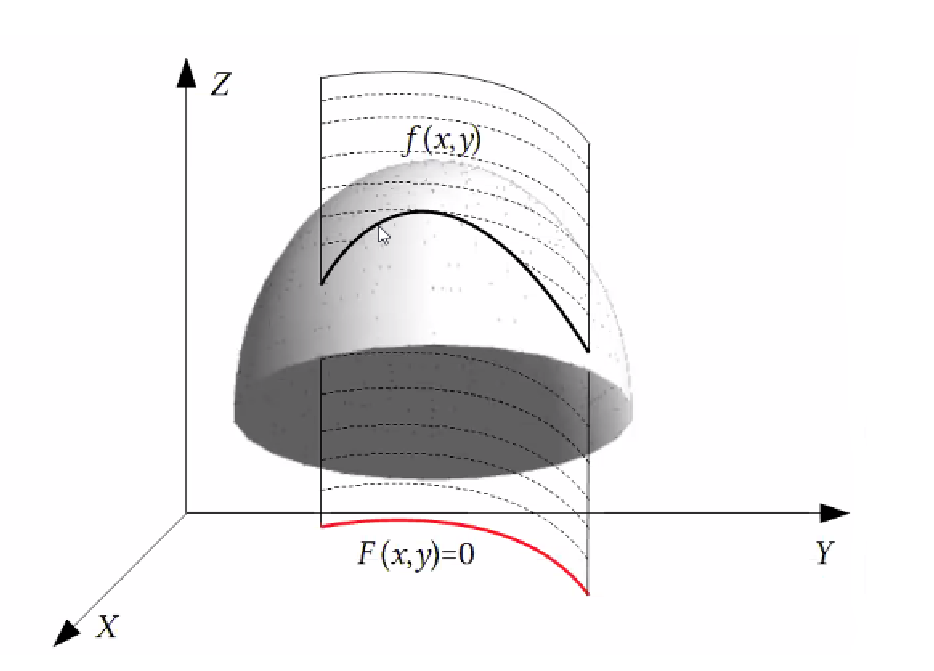
\includegraphics[scale=0.4]{img/rzut_plaszczyznaXY.png}
\end{center}

\begin{przyklad}

\[ f(x,y) = -xy, \ F(x,y) = 2x + y = 0 \]

\begin{center}To daje \ $ y = -2x $ \ czyli\end{center} 
\[ f(x,y) = f(x, -2x) = 2x^2, \ y=-2x, \ x\in \mathbb{R} \]

\begin{center}Czyli zbiór punktów\end{center}
\[ (x, -2x, 2x^2), \ x \in \mathbb{R} \]

Jest to paraboloida ustawiona "pionowo" ale nad prostą \ $ y= -2x $ \ (w płaszczyźnie równoległej do osi $Z$ i zawierającej tą prostą).

\begin{center}
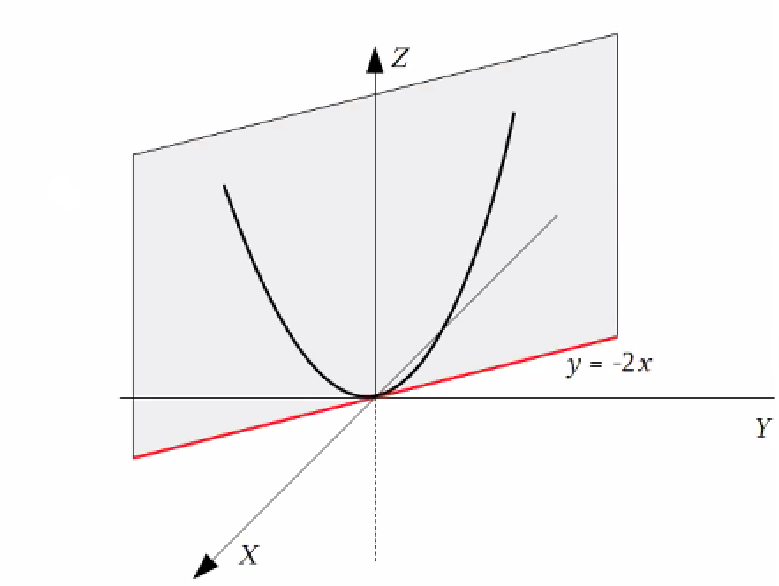
\includegraphics[scale=0.5]{img/paraboloida_przyklad.png}
\end{center}


Ekstrema warunkowe to ekstrema takich funkcji. Liczymy je metodami poznanymi z Analizy Matematycznej 1 (mamy funkcję 1 zmiennej).

W naszym przykładzie mamy do analizy funkcję \ $ f(x) = x^2, \ x \in \mathbb{R} $

Nie trzeba pochodnych, ekstremum to punkt dla \ $x = 0$ -- jest to minimum.

To daje \ $ y = -2 \cdot 0 = 0 $ \ oraz \ $ z = f(0,0) = 0 $ \ więc punkt $ (0,0,0) $.
\end{przyklad}

\subsection*{Wartości największe i najmniejsze funkcji na zadanych zbiorach}

Mamy funkcję \ $ f(x,y), \ D_f = D $

Interesuje nas wartość największa i wartość najmniejsza $f$ na $D$. Te wartości mogą istnieć lub nie. To zależy od funkcji i zbioru.
\bigskip

\begin{tw}{Twierdzenie (Wersja tw. Weiertrassa (AM1) dla funkcji dwóch zmiennych)}

Gdy $D$ jest domknięty (czyli cały brzeg $D$ jest zawarty w $D$) oraz ograniczony (czyli zawiera się w pewnym kole) i $f$ jest ciągła
na $D$ to wartość największa i wartość najmniejsza $f$ na $D$ jest osiągana.
\end{tw}
\bigskip

Gdzie te wartości mogą być osiągane dla funkcji różniczkowalnych?
\begin{itemize}
    \item W punktach stacjonarnych $f$: $ f_x = f_y = 0 $.
    \item Na brzegu $D$: prowadzi to do funkcji warunkowych i ich wartości największych/najmniejszych -- jak dla funkcji jednej zmiennej w AM1
\end{itemize}
\bigskip

Dla punktów z obu przypadków liczymy wartości $f$ i z tych wartości wybieramy najwiekszą i najmniejszą. To daje odpowiedź.

\underline{Uwaga}: Dla punktów stacjonarnych \underline{nie trzeba sprawdzać czy jest to ekstremum}.

Nie potrzeba hesjanu itd. Wystarczy policzyć wartość.
\bigskip

\begin{przyklad}
\[ f(x,y) = xy^2, \ x^2 + y^3 \leq 3 \]

Punkty stacjonarne

$ f_x = y^2 = 0 $

$ f_y = 2xy = 0 $

Wychodzą punkty $ (x, 0) $ oraz $ f(x,0) = \textcolor{magenta}{0} $

Brzeg: \ $ x^2 + y^2 = 3 $. Wystarczy wyliczyć \ $ y^2 = 3 - x^2 $ \ i to daje
\[f(x,y) = f(x) = x(3-x^2) = 3x - x^3, \ x\in \left[-\sqrt3, \sqrt3 \right] \]

Zadanie staje się zadaniem z AM1: znaleźć wartość największą/najmniejszą tej funkcji.

Zatem

\[ f(\pm \sqrt3) = \textcolor{magenta}{0} \]
\[ f' = 3 - 3x^2 = 0 \ \Leftrightarrow \ x = \pm 1 \in \left[ -\sqrt3, \sqrt3 \right] \]
\[ f(-1) = \textcolor{magenta}{-2}, \ f(1) = \textcolor{magenta}{2} \]

Stąd wartość największa to 2, jest osiągana w punktach \ $(1, \sqrt2) $ \ oraz \ $ (1, -\sqrt2) $.

Najmniejsza wartość to -2, jest osiągana w punktach \ $(-1, \sqrt2) $ \ oraz \ $(-1, -\sqrt2) $.
\end{przyklad}


\subsection*{Zadania optymalizacyjne}
\addcontentsline{toc}{subsection}{Zadania optymalizacyjne}

Schemat taki jak w AM1.
\begin{enumerate}
    \item Ułożyć funkcję opisującą daną wielkość.
    \item Znaleźć dziedzinę tej funkcji pasującą do zadania (niekoniecznie dziedzinę naturalną).
    \item Znaleźć wartość największą lub najmniejszą tej funkcji na zadanej dziedzinie.
\end{enumerate}
\bigskip

\begin{przykladbig}

Spośród wszystkich trójkątów o obwodzie równym $3$ jednostki znaleźć ten trójkąt, który ma największe pole.
\medskip

1. Wzór funkcji.

Jeśli boki tego trójkąta mają długości $a,b,c > 0$ to pole jest dane wzorem
\[ S = \sqrt{p(p-a)(p-b)(p-c)} \textrm{ \ gdzie \ } p = \frac{a+b+c}{2} \quad \textrm{(wzór Herona)} \]
\medskip

2. Dziedzina $f$: $ a,b > 0, \ c = 3 - a - b > 0 $ \ oraz z warunku trójkąta

\[ \begin{array}{ccc} 
    a+b>c & \Leftrightarrow & b > 1,5 - a \\
    a+c>b & \Leftrightarrow & 0 < b < 1,5 \\
    b+c>a & \Leftrightarrow & 0 < a < 1,5
\end{array} \]

To daje trójkąt o wierzchołkach w punktach \ $(1.5, \ 0), (0, \ 1.5)$ oraz $(1.5, \ 1.5)$ \ ale bez brzegu.
Aby mieć gwarancję istnienia wartości największej (twierdzenie Weiertrassa) dołączamy brzeg do trójkąta i mamy $D_f$:

\[ 0 \leq a \leq 1,5 \]
\[ 1,5 - a \leq b \leq 1,5 \]

\begin{center}
    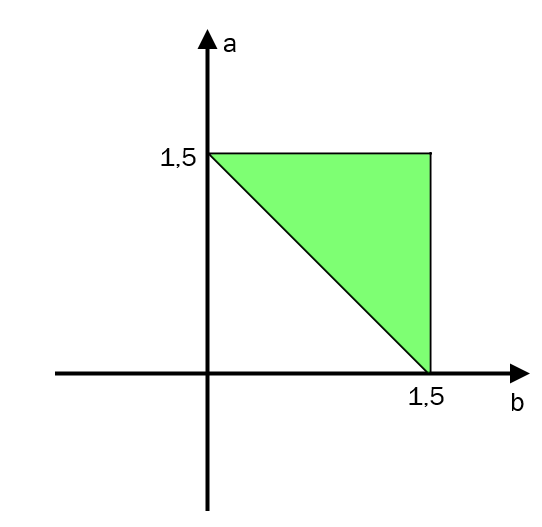
\includegraphics[scale=0.5]{img/trojkat.png}
\end{center}
\bigskip

3.Wartość największa $f$ \bigskip

a) Na brzegu

Brzeg składa się z trzech boków o równaniach
\[ \begin{array}{cc}
    a = 1,5: & f \equiv \textcolor{magenta}{0} \\
    b = 1,5: & f \equiv \textcolor{magenta}{0} \\
    b = 1,5 - a: & f \equiv \textcolor{magenta}{0} \\
\end{array}
\]

To na pewno nie jest wartość największa \bigskip

b) W punktach stacjonarnych we wnętrzu

\[ f(a,b) = \sqrt{1,5(1,5-a)(1,5-b)(a+b-1,5)} \quad \textrm{więc} \]
\[ f_a = \frac{1}{2\sqrt{do poprawy}} \cdot 1,5 \cdot (1,5 - b) \cdot (-(a+b - 1,5) + 1(1,5 - a)) = 0 \]

To daje układ

\[ \begin{cases} (1,5 - b) \cdot (3 - 2a - b) = 0 \\ (1,5 - a) \cdot (3 - 2b - a) = 0 \end{cases} \]

Zatem 

\[ \begin{cases} b = 1,5 \ \textrm{brzeg -- odrzucamy} \ \lor \ 3 - 2a - b = 0 \\
    a = 1,5 \ \textrm{brzeg -- odrzucamy} \ \lor \ 3 - 2b - a = 0
\end{cases} \]

Dla punktów we wnętrzu trójkąta jest więc

\[ 
\begin{cases}
    3 - 2a - b = 0 \\
    3 - 2b - a = 0
\end{cases}    
\]

To daje \ $ a = b = 1$ oraz \ $ f(1,1) = \textcolor{magenta}{\frac{\sqrt3}{4}} $. To jest wartość największa.

Ponadto wtedy $c = 1$. Jest to więc trójkąt równoboczny.
\end{przykladbig}